% Prof. Dr. Ausberto S. Castro Vera
% UENF - CCT - LCMAT - Curso de Ci\^{e}ncia da Computa\c{c}\~{a}o
% Campos, RJ,  2015
% Disciplina: An\'{a}lise e Projeto de Sistemas
% Aluno:


\chapter{Projeto do Sistema}

\chapter{Pontos de Vista do Sistema}

São diferentes formas e perspectivas de enxergar o sistema. O sistema pode ser visto de várias maneiras, sendo eles divididos em grupos para ter uma visão mais clara.

\section {Direto}

Entidades que fornecem informação ao sistema diretamente e recebe informações destes diretamente:

\begin{enumerate}
\item Alunos
\item Professores
\item Gerente de redes
\item Equipe de desenvolvimento
\item Funcionários

\section {Indireto}

O ponto de vista indireto serão as pessoas tem interesse no sistema, porém não trabalham diretamente com o sistema:

\item Governo
\item Área financeira
\item Fornecedores
\item Vestibulando 
\item Área Limpeza
\end{enumerate}

\section {Serviços}
	\subsection {Direto:}
	\begin{enumerate}
	\item Aluno
		\begin{itemize}
		\item Matrícula
		\item Recebimento de bolsa
		\item Biblioteca
		\item Acesso à internet
		\item Úteis escolares
		\end{itemize}
		
	\item Professores
	    \begin{itemize}
		\item Nota
		\item Folha de presença
		\item Plano de aula
		\item Acesso a internet
		\item E-mail personalizado
		\end{itemize}
		
	\item Gerente de redes
		\begin{itemize}
		\item Supervisionamento a rede do servidor
		\item Relatorio das quedas
		\item Manutenção em caso de queda de rede
		\item Coordenar os estagiarios
		\item Negociações
		\end{itemize}
		
	\item Equipe de desenvolvimento
		\begin{itemize}
		\item Desenvolvimento interno do software
		\item Manutenção preventiva
		\item Correções de erro
		\item Otimização do sistema
		\item Atualização do sistema
		\end{itemize}
		
	\item Funcionários
		\begin{itemize}		
		\item Acesso ao contra-cheque
		\item financeiro
		\item Utilização de diversas ferramentas
		\item Responsabilidade
		\item Cumprimento de tarefas
		\end{itemize}
	
	\subsection {Indireto:}
	\item Governo
		\begin{itemize}
		\item Comprovante
		\item Cadastro de Instituições
		\item Elaboração de termos
		\item Emissão de documentos
		\item Validação do sistema
		\end{itemize}
			
	\item Área Financeira
		\begin{itemize}
		\item Contas a receber
		\item Contas a pagar
		\item Boletos bancários
		\item Faturas
		\item Receitas e despesas
		\end{itemize}

						
	\item Fornecedores
		\begin{itemize}
		\item Licitações
		\item Solicitação de Compras
		\item Negociação para o menor preço
		\item Data de renovação da licitação
		\item Notas fiscais
		\end{itemize}
		
	\item Vestibulando
		\begin{itemize}
		\item Informações
		\item Notas Vestibular
		\item Aprovação		
		\item Manifestação de lista de espera
		\item Exclusão
		\end{itemize}
					
	\item Área Limpeza
		\begin{itemize}
		\item Pagamentos
		\item Contra-cheque
		\item Solicitação de 2 via
		\item Estação de trabalho
		\item Férias
		\end{itemize}
		\end{enumerate}
		
\section {Hierarquia de Pontos de Vista}
	
É uma visão organizada e estruturada dos pontos de vista, no qual são mostrados todos os requisitos e pontos de vista do sistema, como mostra a Figura abaixo.
   \begin{figure}[H]
	      \centering
	       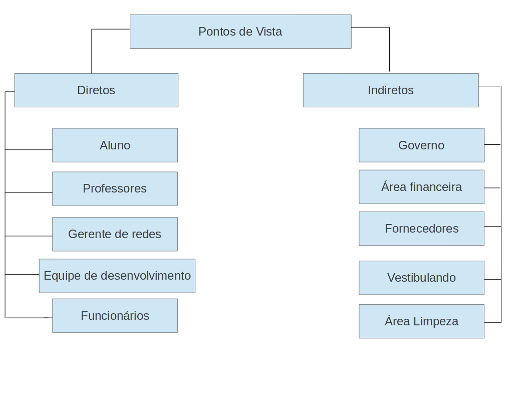
\includegraphics{hierarquia2}
	       \caption{Hierarquia de Pontos de Vista}
	       \label{figRotulo}
               \end{figure}
               
               
    
 \section{Modelagem do Sistema}
 
 É um modelo abstrato do sistema representando uma visão ou perspectiva.
 Para o sistema da empresa SOFT COMPANY são construídos modelos que explicam as características
 e o comportamento de todo o sistema na base de software.
 
   \begin{figure}[H]
	      \centering
	       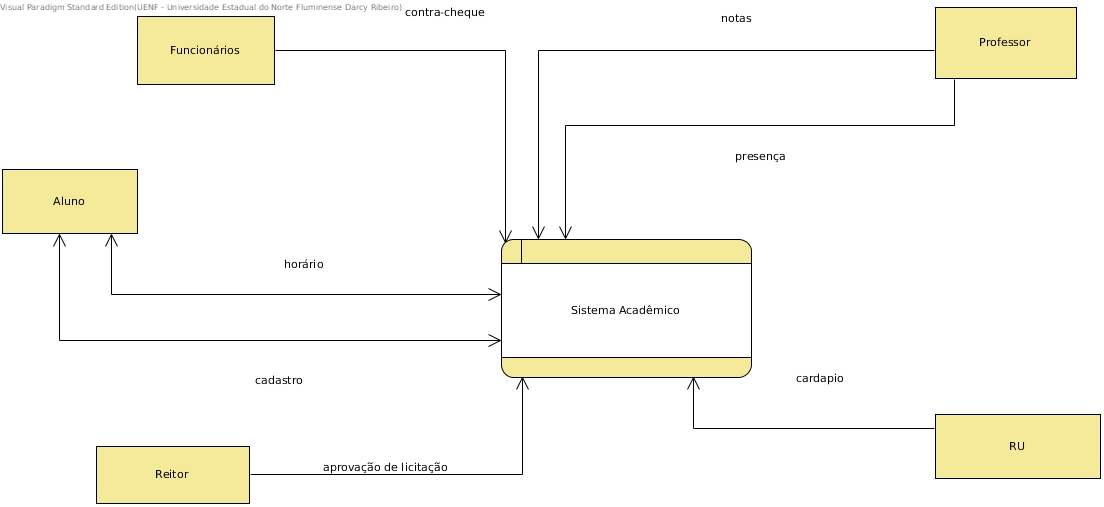
\includegraphics{diagrama1.jpg}
	       \caption{Modelo do sistema}
	       \label{figRotulo}
               \end{figure}
               
               
\section{Entrevista}

  \subsection{Seleção de entrevistados}
  Os entrevistados serão:
Rodolfo da Silva, Aluno, será entrevistado segunda de 8:00 - 10:30
Fernando Barreto, Gerente de Banco de dados, será entrevistado segunda de 11:00 - 12:30
Marco Antônio, Tesoureiro, será entrevistado quarta de 8:30 - 10:30
Jennifer de Souza, Gerente de Relações Públicas, será entrevistada quarta de 11:00 - 12:30
José Cezar, Motorista, será entrevistado quinta de 10:00 – 12:00
Para todos os entrevistados a finalidade da entrevista será saber como o sistema tem modificado o seu trabalho diário.
 
 \subsection{Planejamento das Perguntas: 3 tipos}
 Perguntas fechadas:
		André da Silva
Qual foi, em média, o aumentou da circulação de matérias em termos de entrada e saída diária após a implementação do novo sistema?

Qual foi a redução de tempo médio que aconteceu no processamento de saída e entrada de pedidos depois da automação devido a implementação do novo sistema?

Fernando Barreto
O novo sistema lhe traz transtornos com respeito a travamento, lentidão ou ter que recorrer várias vezes ao backup?

O novo sistema lhe causa transtorno com respeito a tentativas de invasões feito por hackers ou programas maliciosos com o objetivo de corromper os dados?

Marco Antônio
O novo programa é preciso na geração de relatório de lucros?

Você já teve o problema de o dinheiro no total contabilizado ser diferente do calculado pelo programa sendo diferenças discrepantes?

Jennifer de Souza
Após a implementação do novo sistema, tem recebido reclamações dos clientes com respeito ao acesso do programa pela internet ou qualquer tipo de transtorno causa de erros do sistema?

Foi registrado aumento no número de pedidos após implementação dos pedidos online?

José Cezar
O sistema de GPS, resultado da implantação do novo sistema, tem agilizado e facilitado seu trabalho?

O novo sistema lhe atualiza com as coordenadas corretas e com tempo aceitável?

Perguntas Abertas:
Pergunta para todos os entrevistados:
Em sua opinião, o novo sistema tem facilito e agilizado seu trabalho de forma geral?

O que você acha que poderia mudar, ser acrescentado ou retirado, no novo sistema que agilizaria e facilitaria ainda mais o seu trabalho?

Perguntas Analíticas:
Pergunta para todos os entrevistados:
Por que ou Como?
Obs: com relação à primeira e segunda pergunta do conjunto de perguntas abertas.



Pode ser mais específico(a)?
Obs: com relação à segunda pergunta do conjunto de perguntas abertas e caso não for bem explicado pelo entrevistado.

\subsection{Preparação para entrevista}
As perguntas serão feitas na ordem em que foram escritas, porém, irão começar pelas perguntas abertas, depois as perguntas analíticas, por último, as perguntas fechadas. Cada entrevistado possui o seu conjunto de perguntas fechadas com respostas específicas e informações que só ele e os que trabalham na mesma área que ele possuem essas informações. Além de tudo, o entrevistado deverá estar trajando uma roupa social discreta para que ele e o entrevistador possam interagir de forma que fiquem a vontade e possa ser extraída o máximo de informação do entrevistado.
\subsection{Condução da Entrevista}
 Perguntas fechadas:
André da Silva
Qual foi, em média, o aumentou da circulação de matérias em termos de entrada e saída diária após a implementação do novo sistema? 
Resposta: Aumento grandemente, o entra e sai dos produtos usados na empresa está tão grande como o entra e sai de produtos de uma rede de supermercados em que eu já trabalhei.

Qual foi a redução de tempo médio que aconteceu no processamento de saída e entrada de pedidos depois da automação devido a implementação do novo sistema?
Resposta: Estão instantâneos, basta digitar o produto que ele processa a entrada e a saída no mesmo tempo em que apertei o botão, isso também gero uma grande economia de papel visto que quase não usamos mais.

Fernando Barreto
O novo sistema lhe traz transtornos com respeito a travamento, lentidão ou ter que recorrer várias vezes ao backup?
Resposta: Não, ele funciona muito bem.

O novo sistema lhe causa transtorno com respeito a tentativas de invasões feito por hackers ou programas maliciosos com o objetivo de corromper os dados?
Resposta: Não, até hoje não registrei nenhuma tentativa de invasão, mas pela minha análise pessoal do sistema ele é bem seguro.

Marco Antônio
O novo programa é preciso na geração de relatório de lucros?
Resposta: A sim, com certeza, ele contabiliza todos os rendimentos de forma bem precisa e gera um relatório de fácil compreensão.

Você já teve o problema de o dinheiro no total contabilizado ser diferente do calculado pelo programa talvez diferenças discrepantes?
Resposta: Não, eu sempre faço uma checagem para ter certeza se há alguma valor absurdo mas eles estão sempre de acordo com o esperado.


Jennifer de Souza
Após a implementação do novo sistema, tem recebido reclamações dos clientes com respeito ao acesso do programa pela internet ou qualquer tipo de transtorno causa de erros do sistema?
Resposta: Bem poucas, elas diminuíram muitas após a implantação desse novo sistema.

Foi registrado aumento no número de pedidos após implementação dos pedidos online?
Resposta: A com certeza, mesmo com uma pequena diminuição dos pedidos feitos pelo telefone, por causa da preferência de alguns de comprar pela internet, mesmo com isso os pedidos ainda aumentaram muito, acredito que com o site há uma maior divulgação da empresa também.


José Cezar
O sistema de GPS, resultado da implantação do novo sistema, tem agilizado e facilitado seu trabalho?
Resposta: Sim, e muito, visto que antes eu tinha que procurar no mapa o local para levar o caminhão, agora com o GPS fico muito mais prático, sem contar que não preciso voltar para a empresa para pegar novas coordenadas, basta uma atualização que está tudo certo.

O novo sistema lhe atualiza com as coordenadas corretas e com tempo aceitável?
Resposta: Sim, porém, dependendo da localidade pelo sinal de internet não ser dos melhores demora um pouco, mas ainda assim é muito mais rápido do que o antigo esquema que eu seguia.

Perguntas Abertas:
Em sua opinião, o novo sistema tem facilito e agilizado seu trabalho de forma geral?
Respostas:
André da Silva: Absolutamente sim, também do jeito que aumentou a demanda não sei como poderia trabalhar sem ele.

Fernando Barreto: Com certeza, eficiente e seguro, definitivamente o novo sistema foi um bom investimento.

Marco Antônio: Sim e muito, com o sistema de relatórios não fico tão estressado com a possibilidade de erros de cálculos.

Jennifer de Souza: Claro que sim, só de não ter que lidar com as reclamações de antigamente já é um grande alívio.

José Cezar: Facilitou e muito, o trabalho ficou bem menos monótono, e mais fácil visto que o GPS e as novas coordenadas me ajudarem a chegar rapidamente e facilmente ao local certo.

O que você acha que poderia mudar, ser acrescentado ou retirado, no novo sistema que agilizaria e facilitaria ainda mais o seu trabalho?
Respostas:
Todos responderam que o sistema está ótimo ou excelente, com exceção do Fernando Barreto (Gerente de Banco de dados) que respondeu: o sistema está ótimo, porém, como todo sistema se não for feitos upgrades regulares o sistema se torna obsoleto e ineficiente, portanto, minha sugestão é que fação melhorias todo o ano para que o sistema continue como está agora, funcionando de forma rápida e eficiente.

\subsection{Acompanhamento após entrevista: relatório}

Tudo ocorreu como planejado, os entrevistados se sentiram à vontade com o tom da entrevista, responderam de maneira clara e satisfatória, ficando claro de que o sistema foi um excelente investimento e que ele deve continuar e ser melhorado, assim como foi sugerido pelo Gerente de Banco de dados Fernando Barreto, pois pode proporciona um grande aumento na eficiência da empresa e na qualidade do trabalho exercido pelos funcionários de um modo geral, desde de o gerente ao caminhoneiro.

\section{Modelagem do Sistema}
É um modelo abstrato do sistema representando uma visão ou perspectiva. Para o sistema da empresa DECKEL COMPANY são construídos modelos que explicam as características e o comportamento de todo o sistema na base de software.

\subsection{Diagrama de contexto}
Mostra como as partes interessadas e outras entidades (Figura 7.1) interagem com o sistema indicando suas entradas e saídas.
captions(Figura 7.1: Diagrama de Contexto do sistema)

\subsection{Diagrama de Fluxo de Dados}
O DFD é uma técnica usada na programação estruturada de diagramação de software que possui diversos tipos de diagramas, podendo ser derivados em outros diagramas. O diagrama apresenta um modelo de organização do sistema.


\subsection{Entidade de Relacionamento}
É um modelo que mostra as informações que são criadas, armazenadas e usadas pelo sistema.
No diagrama (como mostra a Figura 7.5) está representado um modelo que é usado para ajudar o desenvolvimento de um banco de dados.

\subsection{DFD Físico}
O DFD físico representa o modo como o sistema é implementado fisicamente. Já o DFD lógico representa apenas os processos de negócio, independentemente da maneira como são implementados. A Figura 7.6 representa a implementação de um DFD lógico para um DFD físico.

\subsection{ER Físico}
O ER físico apresenta mais detalhes sobre o ER (Diagrama Entidade-Relacionamento) com informações mais específicas sobre o banco de dados escolhido. Enquanto o ER lógico preocupa-se mais com os conceitos e formas de organização lógica dos dados. A Figura 7.7 representa o modelo do ER físico no Sistema de Caminhão.

\section{Estratégia do Sistema}

\subsection{Desenvolvimento Personalizado}
 O desenvolvimento personalizado é aquele no qual o desenvolvedor dentro da empresa possui o controle total sobre sua a aparência e funcionalidade. O sistema permite ser flexível e criativo na maneira de solucionar problemas operacionais.

\subsection{Sistema Pronto}
Existem muitos sistemas prontos que são comercializados para as empresas, a melhor qualidade desses sistemas são seu curto tempo de prazo, já que muitas vezes o empreendedor necessita do sistema com urgência, economizando muito tempo gasto em sua criação. O sistema a ser escolhido é sempre o que melhor atende as exigências da empresa.

\subsection{Terceirização}
 Esse serviço é utilizado na contratação de um fornecedor, desenvolvedor ou provedor de serviço externo para criar o sistema. Essas pessoas além de serem mais experientes na tecnologia, dispõem de mais recursos humanos qualificados.

\subsection{Estratégia do Projeto}
 Nas tabelas abaixo foram elaboradas os três tipos de Estratégias de Projeto para três situações reais diferentes, sendo que uma delas é o sistema desenvolvido neste documento (Figura 8.1, Figura 8.2 e Figura 8.3).
 
\section{Arquitetura do Sistema}
Na arquitetura são determinadas as necessidades de todas as pessoas envolvidas ou afetadas por qualquer mudança no sistema. É feita uma análise de alto nível nos requisitos do sistema, baseada nas necessidades dos usuários ou de restrições como custos e cronograma.

\subsection{Estilos de Arquitetura}
Arquitetura do Sistema
Possui os componentes de software, suas propriedades externas e seus relacionamentos com outros softwares já existentes, além de estar ligada também com a arquitetura de hardware do sistema. Abaixo são mostrados dois modelos de arquitetura de hardware (Figura 9.3 e Figura 9.4).
Modelo 1 da Arquitetura de Software: